\documentclass[12pt,letterpaper]{article}
\usepackage{graphicx,textcomp}
\usepackage{natbib}
\usepackage{setspace}
\usepackage{fullpage}
\usepackage{color}
\usepackage[reqno]{amsmath}
\usepackage{amsthm}
\usepackage{fancyvrb}
\usepackage{amssymb,enumerate}
\usepackage[all]{xy}
\usepackage{endnotes}
\usepackage{lscape}
\newtheorem{com}{Comment}
\usepackage{float}
\usepackage{hyperref}
\newtheorem{lem} {Lemma}
\newtheorem{prop}{Proposition}
\newtheorem{thm}{Theorem}
\newtheorem{defn}{Definition}
\newtheorem{cor}{Corollary}
\newtheorem{obs}{Observation}
\usepackage[compact]{titlesec}
\usepackage{dcolumn}
\usepackage{tikz}
\usetikzlibrary{arrows}
\usepackage{multirow}
\usepackage{xcolor}
\newcolumntype{.}{D{.}{.}{-1}}
\newcolumntype{d}[1]{D{.}{.}{#1}}
\definecolor{light-gray}{gray}{0.65}
\usepackage{url}
\usepackage{listings}
\usepackage{color}

\definecolor{codegreen}{rgb}{0,0.6,0}
\definecolor{codegray}{rgb}{0.5,0.5,0.5}
\definecolor{codepurple}{rgb}{0.58,0,0.82}
\definecolor{backcolour}{rgb}{0.95,0.95,0.92}

\lstdefinestyle{mystyle}{
	backgroundcolor=\color{backcolour},   
	commentstyle=\color{codegreen},
	keywordstyle=\color{magenta},
	numberstyle=\tiny\color{codegray},
	stringstyle=\color{codepurple},
	basicstyle=\footnotesize,
	breakatwhitespace=false,         
	breaklines=true,                 
	captionpos=b,                    
	keepspaces=true,                 
	numbers=left,                    
	numbersep=5pt,                  
	showspaces=false,                
	showstringspaces=false,
	showtabs=false,                  
	tabsize=2
}
\lstset{style=mystyle}
\newcommand{\Sref}[1]{Section~\ref{#1}}
\newtheorem{hyp}{Hypothesis}

\title{Problem Set 2}
\date{Due: October 22, 2026}
\author{Applied Stats/Quant Methods 1}

\begin{document}
	\maketitle
	\section*{Instructions}
\begin{itemize}
	\item Please show your work! You may lose points by simply writing in the answer. If the problem requires you to execute commands in \texttt{R}, please include the code you used to get your answers. Please also include the \texttt{.R} file that contains your code. If you are not sure if work needs to be shown for a particular problem, please ask.
	\item Your homework should be submitted electronically on GitHub.
	\item This problem set is due before 23:59 on Thursday October 22, 2026. No late assignments will be accepted.

\end{itemize}

	
	\vspace{.5cm}
	\section*{Question 1: Political Science}
		\vspace{.25cm}
	The following table was created using the data from a study run in a major Latin American city.\footnote{Fried, Lagunes, and Venkataramani (2010). ``Corruption and Inequality at the Crossroad: A Multimethod Study of Bribery and Discrimination in Latin America. \textit{Latin American Research Review}. 45 (1): 76-97.} As part of the experimental treatment in the study, one employee of the research team was chosen to make illegal left turns across traffic to draw the attention of the police officers on shift. Two employee drivers were upper class, two were lower class drivers, and the identity of the driver was randomly assigned per encounter. The researchers were interested in whether officers were more or less likely to solicit a bribe from drivers depending on their class (officers use phrases like, ``We can solve this the easy way'' to draw a bribe). The table below shows the resulting data.

\newpage
\begin{table}[h!]
	\centering
	\begin{tabular}{l | c c c }
		& Not Stopped & Bribe requested & Stopped/given warning \\
		\\[-1.8ex] 
		\hline \\[-1.8ex]
		Upper class & 14 & 6 & 7 \\
		Lower class & 7 & 7 & 1 \\
		\hline
	\end{tabular}
\end{table}

\begin{enumerate}
	
	\item [(a)]
	Calculate the $\chi^2$ test statistic by hand/manually (even better if you can do "by hand" in \texttt{R}).\\	
	\lstinputlisting[language=R, firstline=44, lastline=67]{PS02_PT.R} 
	\begin{verbatim}
	[1] 3.791168	
	\end{verbatim}
	\lstinputlisting[language=R, firstline=67, lastline=76]{PS02_PT.R} 
	\begin{verbatim}
	[1] 3.791168
	\end{verbatim}
	\lstinputlisting[language=R, firstline=76, lastline=79]{PS02_PT.R} 
	\begin{verbatim}
	[1] TRUE	
	\end{verbatim}
	
	\item [(b)]
	Now calculate the p-value from the test statistic you just created (in \texttt{R}).\footnote{Remember frequency should be $>$ 5 for all cells, but let's calculate the p-value here anyway.}  What do you conclude if $\alpha = 0.1$?\\
		\lstinputlisting[language=R, firstline=86, lastline=87]{PS02_PT.R} 
	\begin{verbatim}
	[1] 0.1502306	
	\end{verbatim}
	\lstinputlisting[language=R, firstline=89, lastline=90]{PS02_PT.R} 
	\begin{verbatim}
	[1] 0.1502306
	\end{verbatim}
	\textbf {We cannot reject the null hypothesis because the pval is greater than our alpha of 0.1.}

	\item [(c)] Calculate the standardized residuals for each cell and put them in the table below.
	
\textbf {The formula for adjusted residual is (fo - fe)/se and se = sqrt(fe(1 - (row total/total))*(1 - (column total/total))). using these formulas we can plug in our variables used in 1a, or the numbers directly as well. Afterwards I will check my answers by comparing both results, and by extracting the standardized residuals from a chi squared test.}
	
	
		\lstinputlisting[language=R, firstline=115, lastline=123]{PS02_PT.R} 
	\begin{verbatim}
	           [,1]      [,2]      [,3]
	[1,]  0.3220306 -1.641957  1.523026
	[2,] -0.3220306  1.641957 -1.523026
	\end{verbatim}
			\lstinputlisting[language=R, firstline=125, lastline=133]{PS02_PT.R} 
	\begin{verbatim}
		[,1]      [,2]      [,3]
		[1,]  0.3220306 -1.641957  1.523026
		[2,] -0.3220306  1.641957 -1.523026
	\end{verbatim}
				\lstinputlisting[language=R, firstline=135, lastline=135]{PS02_PT.R} 
	\begin{verbatim}
     [,1] [,2] [,3]
[1,] TRUE TRUE TRUE
[2,] TRUE TRUE TRUE
	\end{verbatim}
	
					\lstinputlisting[language=R, firstline=137, lastline=137]{PS02_PT.R} 
	\begin{verbatim}
           [,1]      [,2]      [,3]
[1,]  0.3220306 -1.641957  1.523026
[2,] -0.3220306  1.641957 -1.523026
Warning message:
In chisq.test(bribes) : Chi-squared approximation may be incorrect
	\end{verbatim}
	\begin{table}[h]
		
		\centering
		\begin{tabular}{l | c c c }
			& Not Stopped & Bribe requested & Stopped/given warning \\
			\\[-1.8ex] 
			\hline \\[-1.8ex]
			Upper class & 0.3220306 & -1.641957 & 1.523026  \\
			\\
			Lower class & -0.3220306 & 1.641957 & -1.523026  \\
			
		\end{tabular}
	\end{table}
	
	

	\item [(d)] How might the standardized residuals help you interpret the results? 
	
	
	\textbf {The standardized residuals show us that the lower class drivers were asked for bribes more often than we would have expected and the upper class drivers show the opposite. We can see this by looking at their distance away from 0, with positive indicating that the driver was asked more often than expected, and negative indicating less often. We can also see that the residuals for "not stopped" is by far the lowest which indicates that class does not have much of an effect on whether or not you get pulled over. We also know that in a normal distribution most values will fall between -1.96 and 1.96 with a failure to reject the null hypothesis. all of the values we found do fall within those values, which is consistent with our failure to reject the null hypothesis.} 
	
\end{enumerate}
\newpage

\section*{Question 2: Economics}
Chattopadhyay and Duflo were interested in whether women promote different policies than men.\footnote{Chattopadhyay and Duflo. (2004). ``Women as Policy Makers: Evidence from a Randomized Policy Experiment in India. \textit{Econometrica}. 72 (5), 1409-1443.} Answering this question with observational data is pretty difficult due to potential confounding problems (e.g. the districts that choose female politicians are likely to systematically differ in other aspects too). Hence, they exploit a randomized policy experiment in India, where since the mid-1990s, $\frac{1}{3}$ of village council heads have been randomly reserved for women. A subset of the data from West Bengal can be found at the following link: \url{https://raw.githubusercontent.com/kosukeimai/qss/master/PREDICTION/women.csv}\\

\noindent Each observation in the data set represents a village and there are two villages associated with one GP (i.e. a level of government is called "GP"). Figure~\ref{fig:women_desc} below shows the names and descriptions of the variables in the dataset. The authors hypothesize that female politicians are more likely to support policies female voters want. Researchers found that more women complain about the quality of drinking water than men. You need to estimate the effect of the reservation policy on the number of new or repaired drinking water facilities in the villages.
\vspace{.5cm}
\begin{figure}[h!]
	\caption{\footnotesize{Names and description of variables from Chattopadhyay and Duflo (2004).}}
	\vspace{.5cm}
	\centering
	\label{fig:women_desc}
	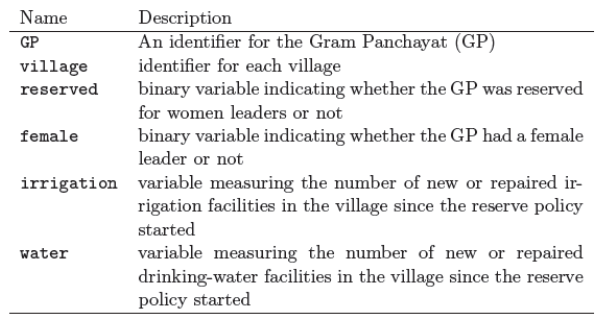
\includegraphics[width=.8\textwidth]{women_desc.png}
	
\end{figure}		

\newpage
\begin{enumerate}
	\lstinputlisting[language=R, firstline=159, lastline=159]{PS02_PT.R} 
	\item [(a)] State a null and alternative (two-tailed) hypothesis.
	 
	\textbf {NULL Hypothesis: Ho Beta = 0}
	
	\textbf {The reserved seats for women in GP have no effect on the number of new or repaired drinking water facilities.}
		
		
	\textbf {Alternative hypothesis (two sided): Ha Beta != 0}
	
	\textbf {The reserved seats for women in GP have an effect on the number of new or repaired drinking water facilities.}
	\item [(b)] Run a bivariate regression to test this hypothesis in \texttt{R} (include your code!).
	
		\lstinputlisting[language=R, firstline=195, lastline=198]{PS02_PT.R} 
		\begin{verbatim}
	Call:
	lm(formula = water ~ reserved, data = GP_women)
	
	Residuals:
	Min      1Q  Median      3Q     Max 
	-23.991 -14.738  -7.865   2.262 316.009 
	
	Coefficients:
	Estimate Std. Error t value       Pr(>|t|)    
	(Intercept)   14.738      2.286   6.446 0.000000000422 ***
	reserved       9.252      3.948   2.344         0.0197 *  
	---
	Signif. codes:  0 ‘***’ 0.001 ‘**’ 0.01 ‘*’ 0.05 ‘.’ 0.1 ‘ ’ 1
	
	Residual standard error: 33.45 on 320 degrees of freedom
	Multiple R-squared:  0.01688,	Adjusted R-squared:  0.0138 
	F-statistic: 5.493 on 1 and 320 DF,  p-value: 0.0197
		\end{verbatim}
	\textbf {p is less than 0.05 so we reject the NULL hypothesis.}
	
	\item [(c)] Interpret the coefficient estimate for reservation policy. 
	
			\lstinputlisting[language=R, firstline=231, lastline=232]{PS02_PT.R} 
	\begin{verbatim}
             Estimate Std. Error  t value           Pr(>|t|)
(Intercept) 14.738318   2.286300 6.446363 0.0000000004216474
reserved     9.252423   3.947746 2.343723 0.0197039791691662
	\end{verbatim}
	
		\textbf {14.738 is intercept, 9.252 is the slope, 0.0197 is the pval}
			
	\textbf {The villages with their GP reserved for a woman leader produced an increase of about 9.25 drinking water facilities on average. About 24 were produced in the GP reserved for women vs 15 in the GP without. Because the reservation effect was randomly assigned, it can be read that this is the effect of the reservation policy. The p-value of 0.0197 supports the alternative hypothesis that reserved seats for women in GP would result in an increase in drinking water facilities as it is less than 0.05. It is worth noting, however, that it appears that the values for the women reserved GPs are being strongly drawn upwards by a handful of villages with very large residuals. The median of the villages without reserved seats is noticeably higher than than those with reserved villages. The outliers, however, draw the mean of the reserved villages higher. As mentioned previously, the random assignment makes it likely that the results are still causal, however the result should be taken cautiously and not seen as conclusive evidence.}
	
\end{enumerate}


%\end{enumerate}
\end{document}
